\documentclass[]{IEEEtran}
% Your packages go here
\usepackage[utf8]{inputenc}
\usepackage{graphicx}
\usepackage{grffile}
\usepackage{gensymb}
\usepackage{amsmath}
\usepackage{amssymb}
\usepackage{listings}
\usepackage{mathtools}
\usepackage{subfig}
\usepackage{xcolor}
\usepackage{multirow}

\usepackage{amsmath}

\DeclareMathOperator{\atantwo}{atan2}

\DeclareMathOperator{\arctantwo}{arctan2}


\definecolor{codegreen}{rgb}{0,0.6,0}
\definecolor{codegray}{rgb}{0.5,0.5,0.5}
\definecolor{codepurple}{rgb}{0.58,0,0.82}
\definecolor{backcolour}{rgb}{0.95,0.95,0.92}

\lstdefinestyle{mystyle}{
    backgroundcolor=\color{backcolour},   
    commentstyle=\color{codegreen},
    keywordstyle=\color{magenta},
    numberstyle=\tiny\color{codegray},
    stringstyle=\color{codepurple},
    basicstyle=\ttfamily\footnotesize,
    breakatwhitespace=false,         
    breaklines=true,                 
    captionpos=b,                    
    keepspaces=true,                 
    numbers=left,                    
    numbersep=5pt,                  
    showspaces=false,                
    showstringspaces=false,
    showtabs=false,                  
    tabsize=2
}
 
\lstset{style=mystyle}
 
\usepackage{lipsum}% http://ctan.org/pkg/lipsum
\usepackage{graphicx}% http://ctan.org/pkg/graphicx

\def\footnoterule{\relax%
  \kern-2pt
  \hbox to \columnwidth{\hfill\vrule width 0.7\columnwidth height 0.4pt\hfill}
  \kern4.6pt}
\makeatother

\renewcommand{\lstlistingname}{Algorithm}% Listing -> Algorithm
\usepackage[noadjust]{cite}
\markboth{MO435 - Probabilistic Machine Learning }{}

\begin{document}

\title{Project 1 }
\author{Ivan Lima do Espirito Santo \thanks{RA: 956694 - i956694@g.unicamp.br}\\ Rosa Yuliana Gabriela Paccotacya Yanque \thanks{RA: 263068 - r263068@dac.unicamp.br} \\ Thiago Gomes Marçal Pereira \thanks{RA: 189691 - t189691@g.unicamp.br}}


\maketitle
  
\begin{abstract}

Nowadays, ...

\end{abstract}
  
\section{Introduction}
\label{sec:introduction}

The task of ...

Since the task ...Figure ~\ref{fig:slam} show some results of this technique~\cite{Zivkovic2004ImprovedAG}.


\begin{figure}[!ht]
  \centering
  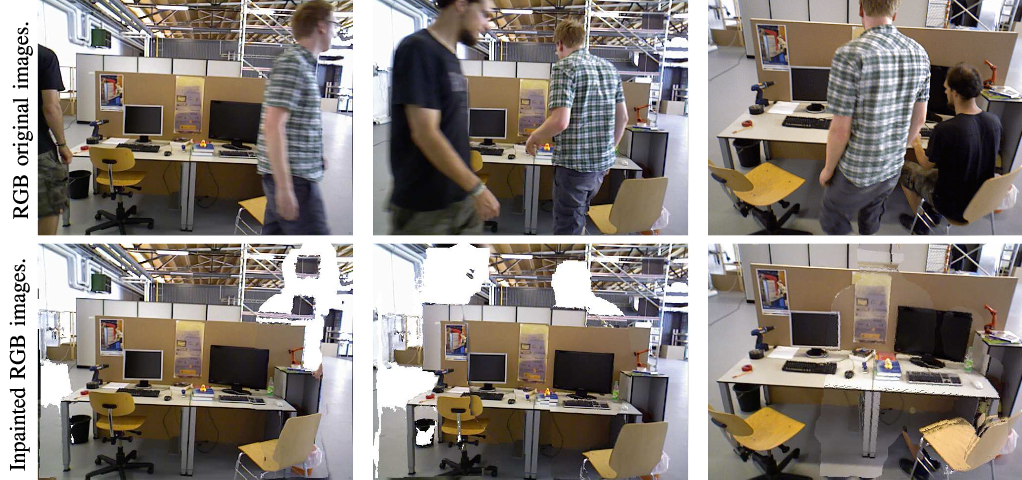
\includegraphics[width=0.46\textwidth]{images/SLAM.png}
  \caption{Results of SLAM inpainting in dynamic scenes.}
  \label{fig:slam}
\end{figure}

The code used in this project was implemented using Python 3.7.3. Table~\ref{tab:software} summarizes the libraries utilized in this work and its respective versions.

\renewcommand{\arraystretch}{1.2}
\begin{table}[h]
    \begin{center}
        \small
        \begin{tabular}{| c | c |} 
            \hline
            \textbf{Library} & \textbf{Version}\\ 
            \hline \hline
            Python & 3.7.3 \\  
            \hline
            NumPy & 1.17.0 \\  
            \hline
        \end{tabular}
    \caption{Python libraries used in this project.}
    \label{tab:software}
    \end{center}
\end{table}

The present report is organized as follows. First, a introduction was done in this section mentioning some related works. The following sections will explain in detail, the procedures followed during the experiments for each section in the pipeline.

\section{Methodology}
\label{sec:methodology}

In this section we present two approaches to address the problem of 

\subsection{First approach}
\label{sec:first_approach}

\begin{figure}[!ht]
  \centering
  \subfloat[]{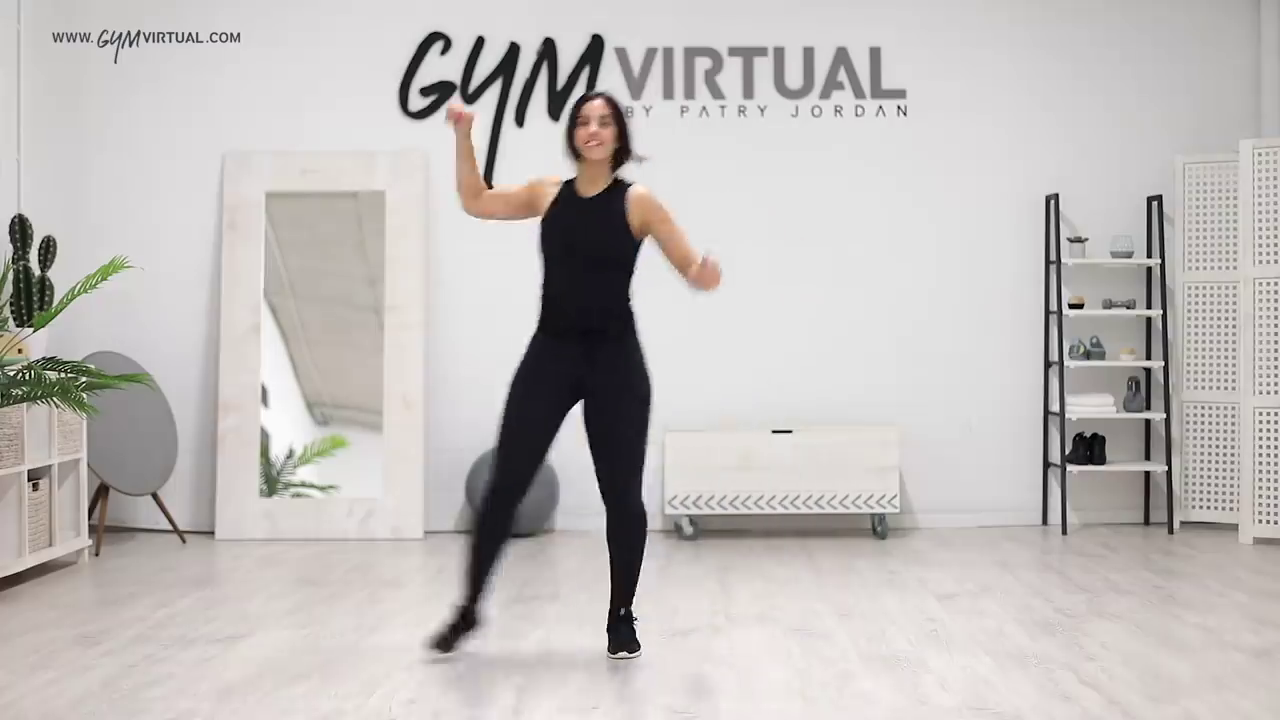
\includegraphics[width=0.22\textwidth]{images/p_0.png}}
  \hspace{1mm}
  \subfloat[]{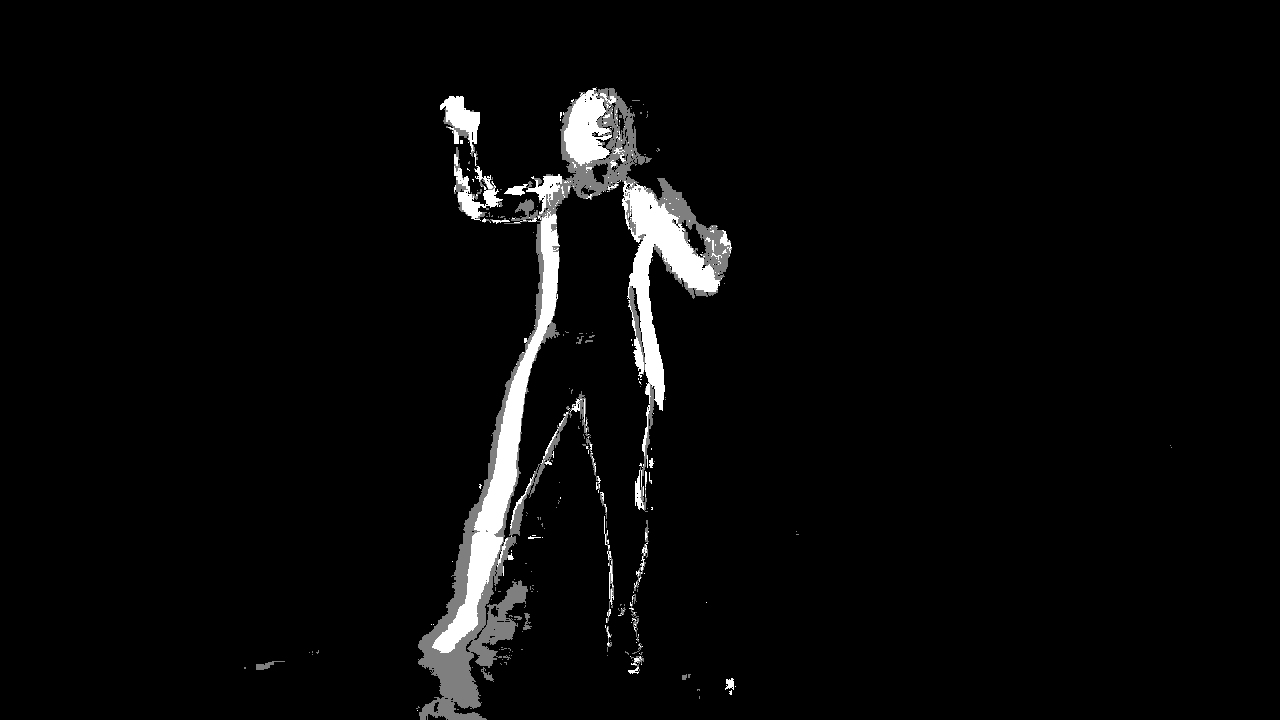
\includegraphics[width=0.22\textwidth]{images/p_1.png}}
  \hspace{1mm}
  \break
  \subfloat[]{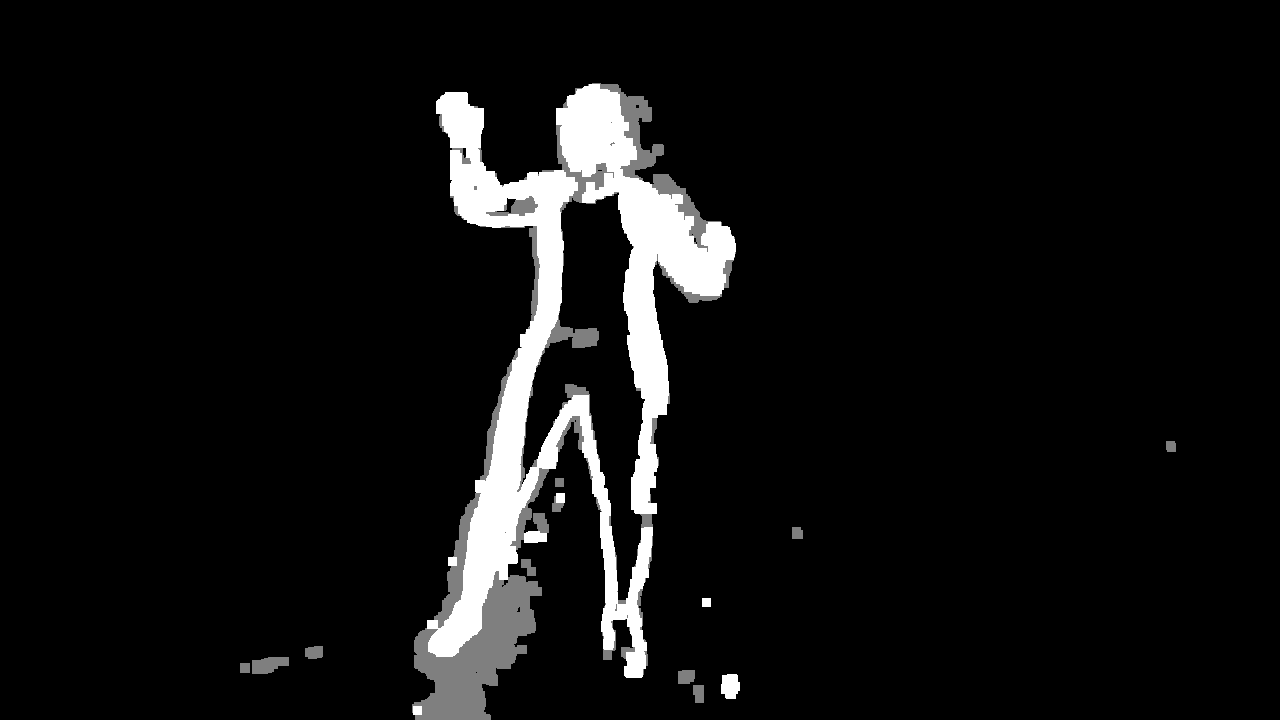
\includegraphics[width=0.22\textwidth]{images/p_2.png}}
  \hspace{1mm}
  \subfloat[]{
\includegraphics[width=0.22\textwidth]{images/p_3.png}}
  \hspace{1mm}
  \caption{(a) Original frame (b) Background subtraction (c) Application of morphological transformations to define the object contour (dilation and erosion) (d) Object filling.}
  \label{fig:gmx}
\end{figure}

\subsection{Second approach}
\label{sec:second_approach}

In this approach, we first created a...
Our objective is to ...  For this purpose, we employ the.

Next, we perform ..

\section{Experiments}

\subsection{First Approach}

\section{Future Work}

\section{Discussion and Conclusions}


\bibliographystyle{abbrv}
\bibliography{bibliography}

\clearpage
\onecolumn
\begin{appendices}

\section{Results of experiments using the second approach}
\label{sec:appendix}

\end{appendices}

\end{document}


